\section{Proposed software architecture}
\label{sec:Proposed software architecture}



% \subsection{Overview}



\subsection{System architecture choice}
The system is build up by several different system architectures.
The over all system architecture is the \textbf{client server architecture} (figure ~\ref{fig:System architecture}) utilizing the \textbf{distributed architecture} using the REST communication interface separating  the main components of our program, the clients and the web server.

\paragraph{Advantages of server client architecture}
\begin{itemize}
	\item By keeping the coupling to the sever very light, other developers can easily use our server(api) to build their own clients. \\
	\item The server is distributed across a network allowing many users to utilize our service.
	\item Users can use all or parts of our API through the REST interface making it very customizable to the users needs.
\end{itemize}
\paragraph{Disadvantages of server client architecture}
\begin{itemize}
	\item The system is distributed which raises a lot of both safety and failure points eg. concurrency.  \\
	\item The solutions performance is heavily relying on the network speed and reliability.  
\end{itemize}

\begin{figure}[H]
\begin{center}
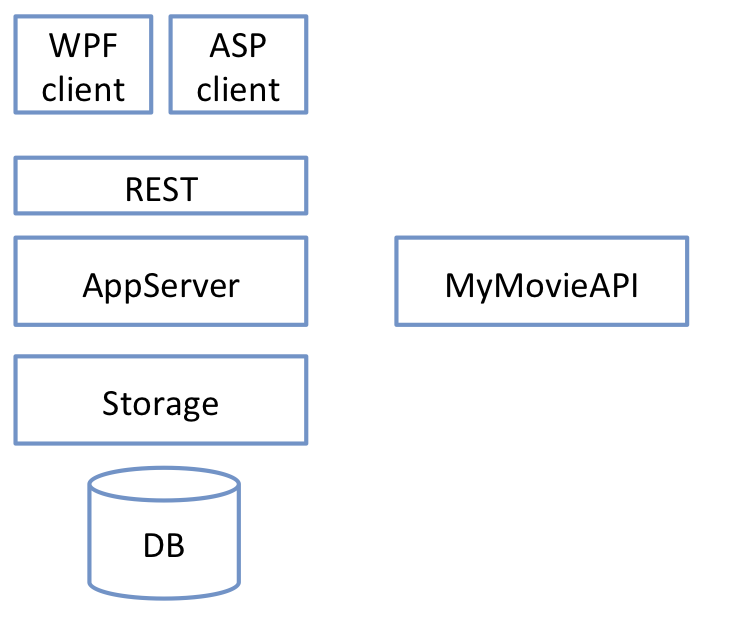
\includegraphics[scale=0.7]{img/SDD/bdsaproject.png}
\caption{System architecture}
\label{fig:System architecture}
\end{center}
\end{figure}

For the different system components we use different internal software architectures. The web server is designed as a layered architecture. On top the REST communication, then a logic layer, than a storage layer and on the bottom concrete persistent modules (eg. A database).

The ASP.net client utilises the Model-View-Controller system architecture, separating presentation and interaction from system data.

\paragraph{Advantages of MVC}
\begin{itemize}
	\item By keeping the visuals separated from the application data, we can achieve very loose coupling, as well as the ability to easily change the same data from many different views, for example via our desktop and web-based clients. 
	\item If there's ever need to change parts of the program, it will be easy to switch out parts of the code.
\end{itemize}
\paragraph{Disadvantages of MVC}
\begin{itemize}
	\item We will most likely have a larger amount of classes than necessary for a project of this scope. 
	\item The class hierarchy might become messier, as we will need a larger amount of classes for simple tasks. \\
\end{itemize}


The WPF client uses the Model-View-Viewmodel (MVVM) pattern, which is a specialization of the MVC pattern. The advantages and disadvantages are the same. Instead of a Controller, it has the ViewModel, which combines properties for databinding by the View and logic like commands.



\subsection{Design pattern choices}
We will in this section document the design patterns utilized by the program. We will mention the reasoning behind our choices.

\begin{itemize}
	\item The \emph{Database Mapper} pattern has been applied when performing transactions between the web server and the database. The system contains a facade exposed to the web server. The facade can be injected with the wanted mapper, which will then connect to the database based on the mapper.
	\item The \emph{Abstract factory} is used in the storage subsystem to create instances of storage. By using this design pattern, we give the subsystem added extendability, simplifying the progress of making plugins that utilize the subsystem.
	\item \emph{Bridge pattern} is implemented in the storage and is used to easily allow the rest of the system to use the data, independent of how the actual storage functionality works, whether it's a relational Database, flatfile, in-memory etc.
	\item The \emph{Adapter pattern} has been used when translating alien movie data from other databases to the format used in the main database.
	\item The \emph{Front Controller Pattern} is used when processing requests. Incoming requests is sent through a delegator to the relevant request controller. The controller determines how the request will affect the database. This allows for new request types to be implemented easily.
	\item The \emph{Facade Pattern} is used for each of the subsystems in the program. All subsystems expose a single facade to be accessed by other subsystems, allowing simpler communication between all of the components in the system. Furthermore the pattern allows each subsystem to be self-contained allowing for inner changes to be made frequently as long as the changes does not change the functionality of the facade.
	\item The \emph{Command Pattern} has been used to invoke delegates in the ViewModels bound by controllers in the Views. A button, for example, will be bound to a command in the ViewModel, and hence code can be executed by the hand of the user.
\end{itemize}

\subsection{Subsystem decomposition}
\label{sec:Subsystem decomposition}
We have grouped our classes into subsystems to create a clearer structure of the program. In this section, we will first show an overview of how the subsystems interact, and then a detailed look at the individual subsystems.\\


\begin{figure}[H]
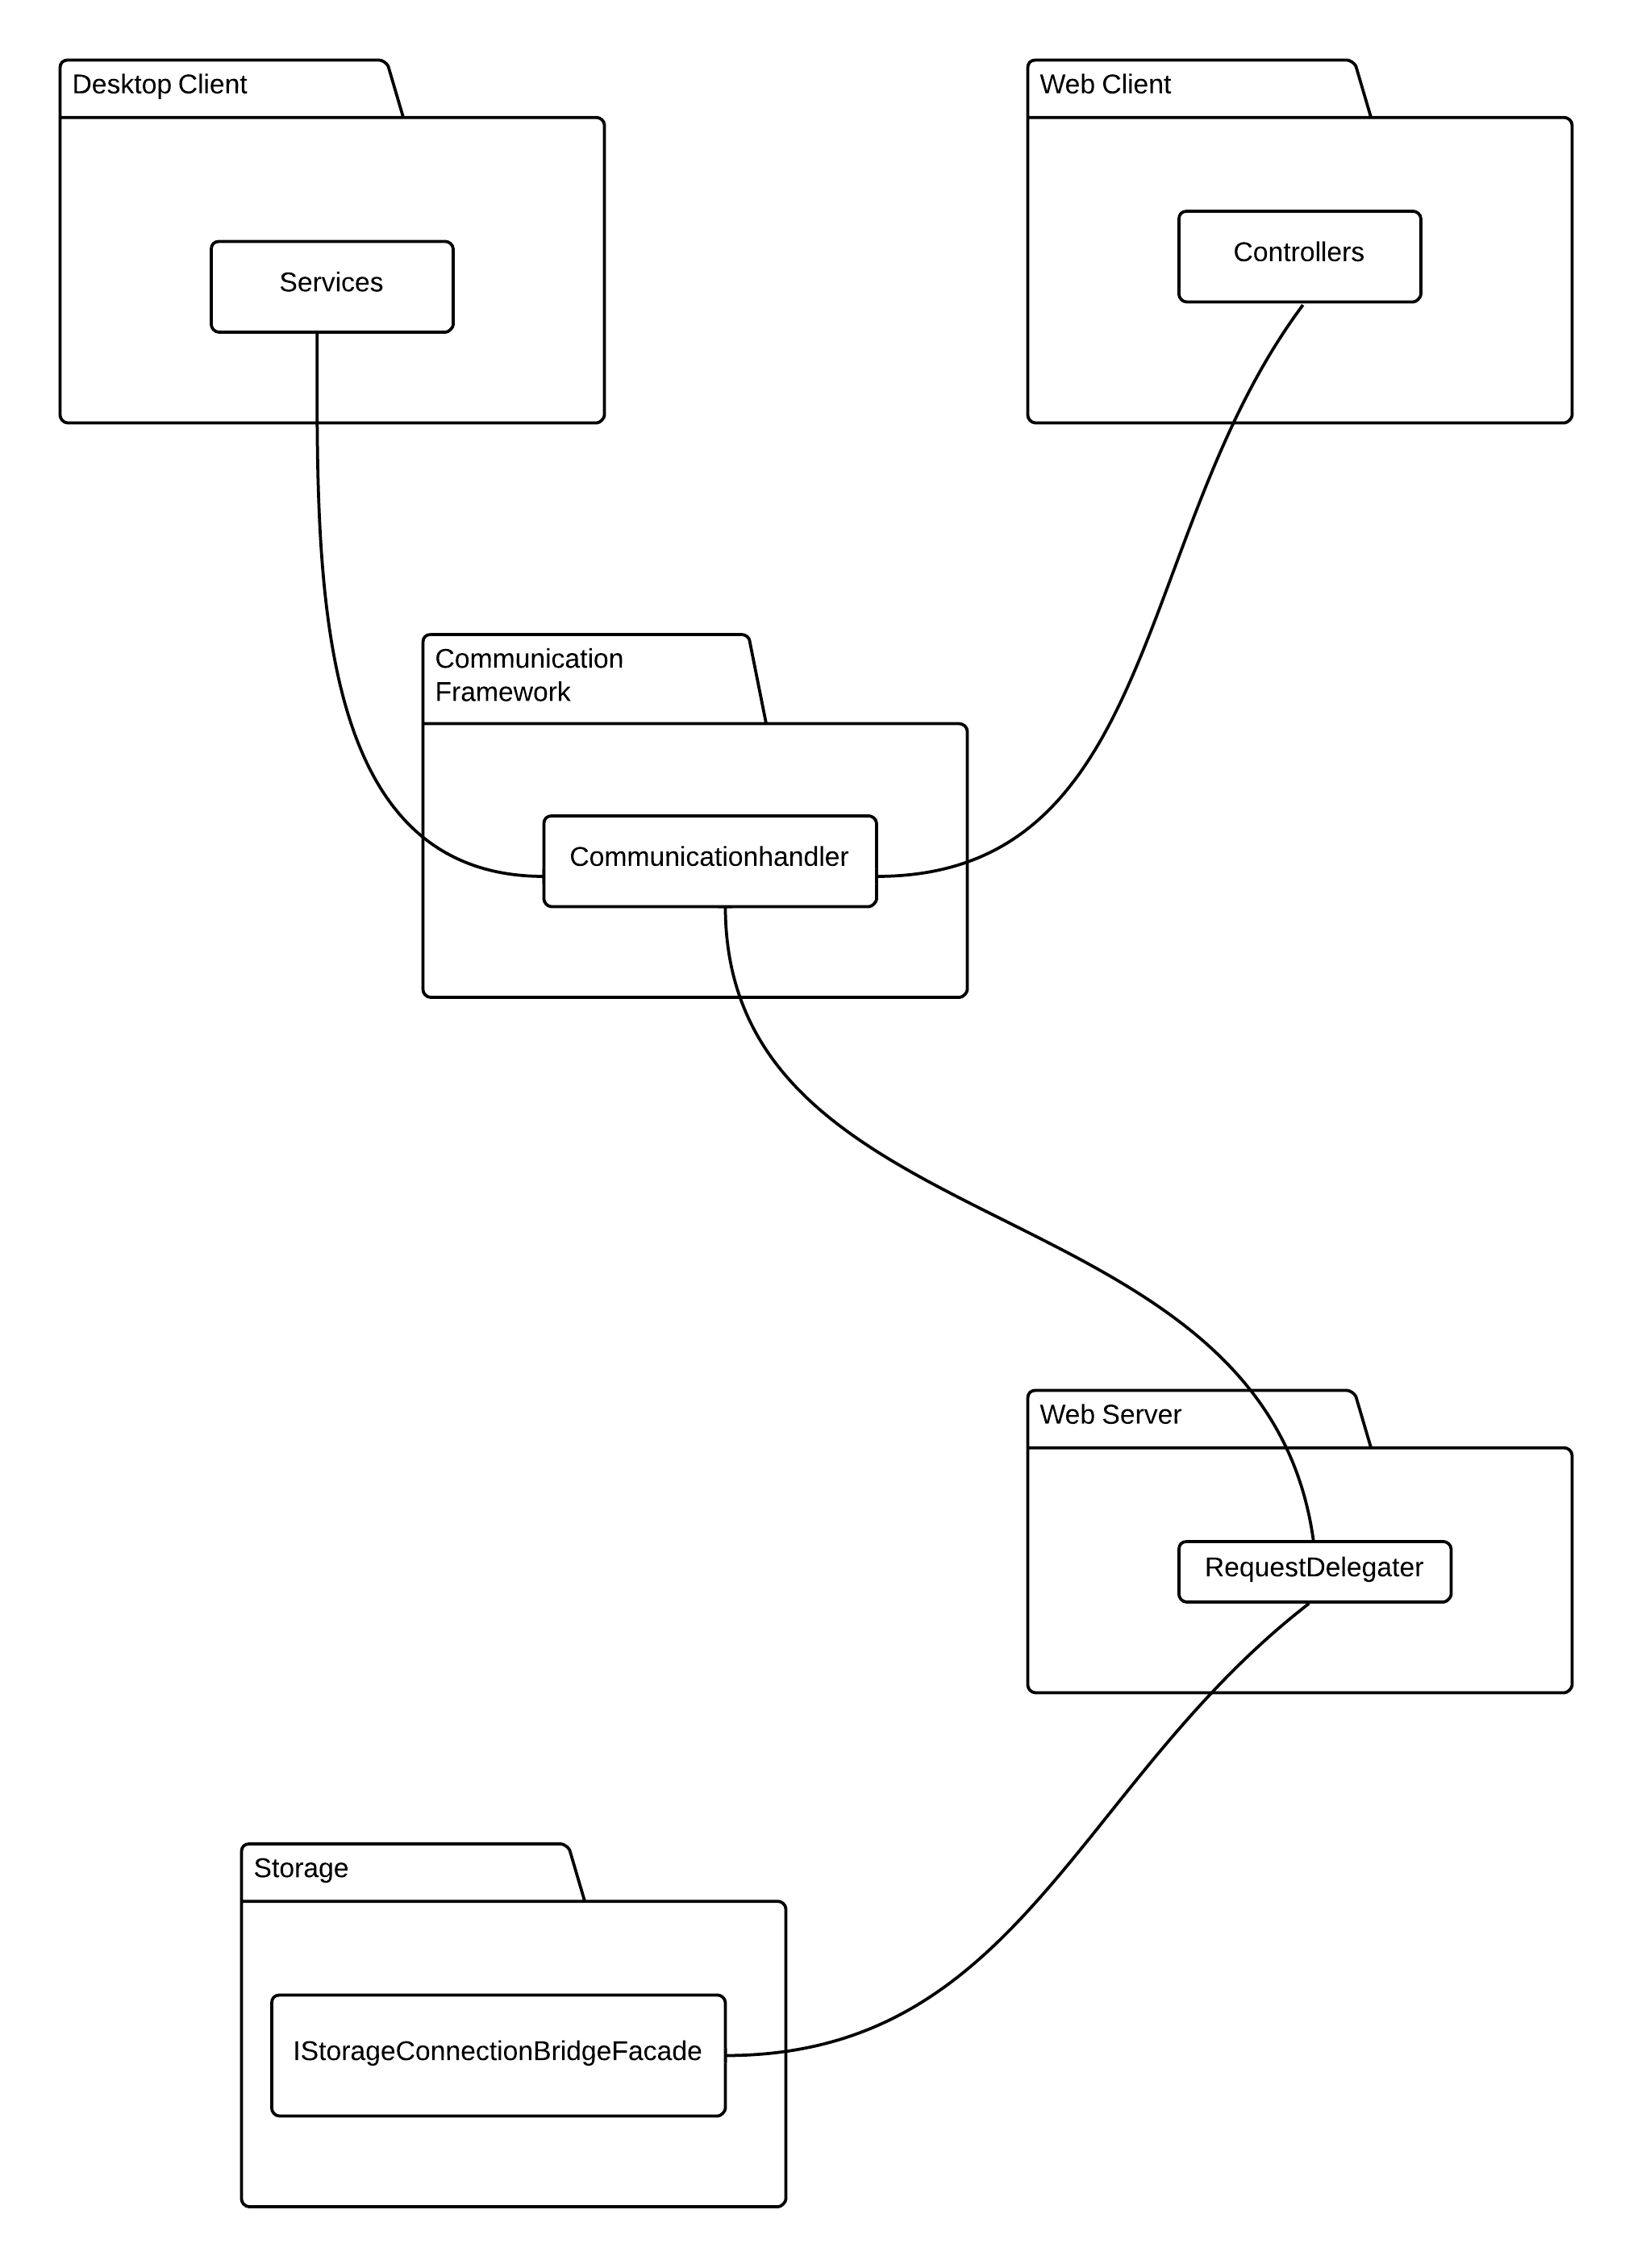
\includegraphics[scale=0.17]{img/SDD/FakeIMDbSubsytems.png}
\caption{Fake IMDb Subsystems}
\label{fig:FakeIMDBSubsystems}
\end{figure}

The software is divided into five main subsystems with one subsystem for each different clients, communicating with the WebServer subsystem through the Communication Framework subsystem. The WebServer subsystem use the Storage subsystem to get/put data to/from the clients.\\


\begin{figure}[H]
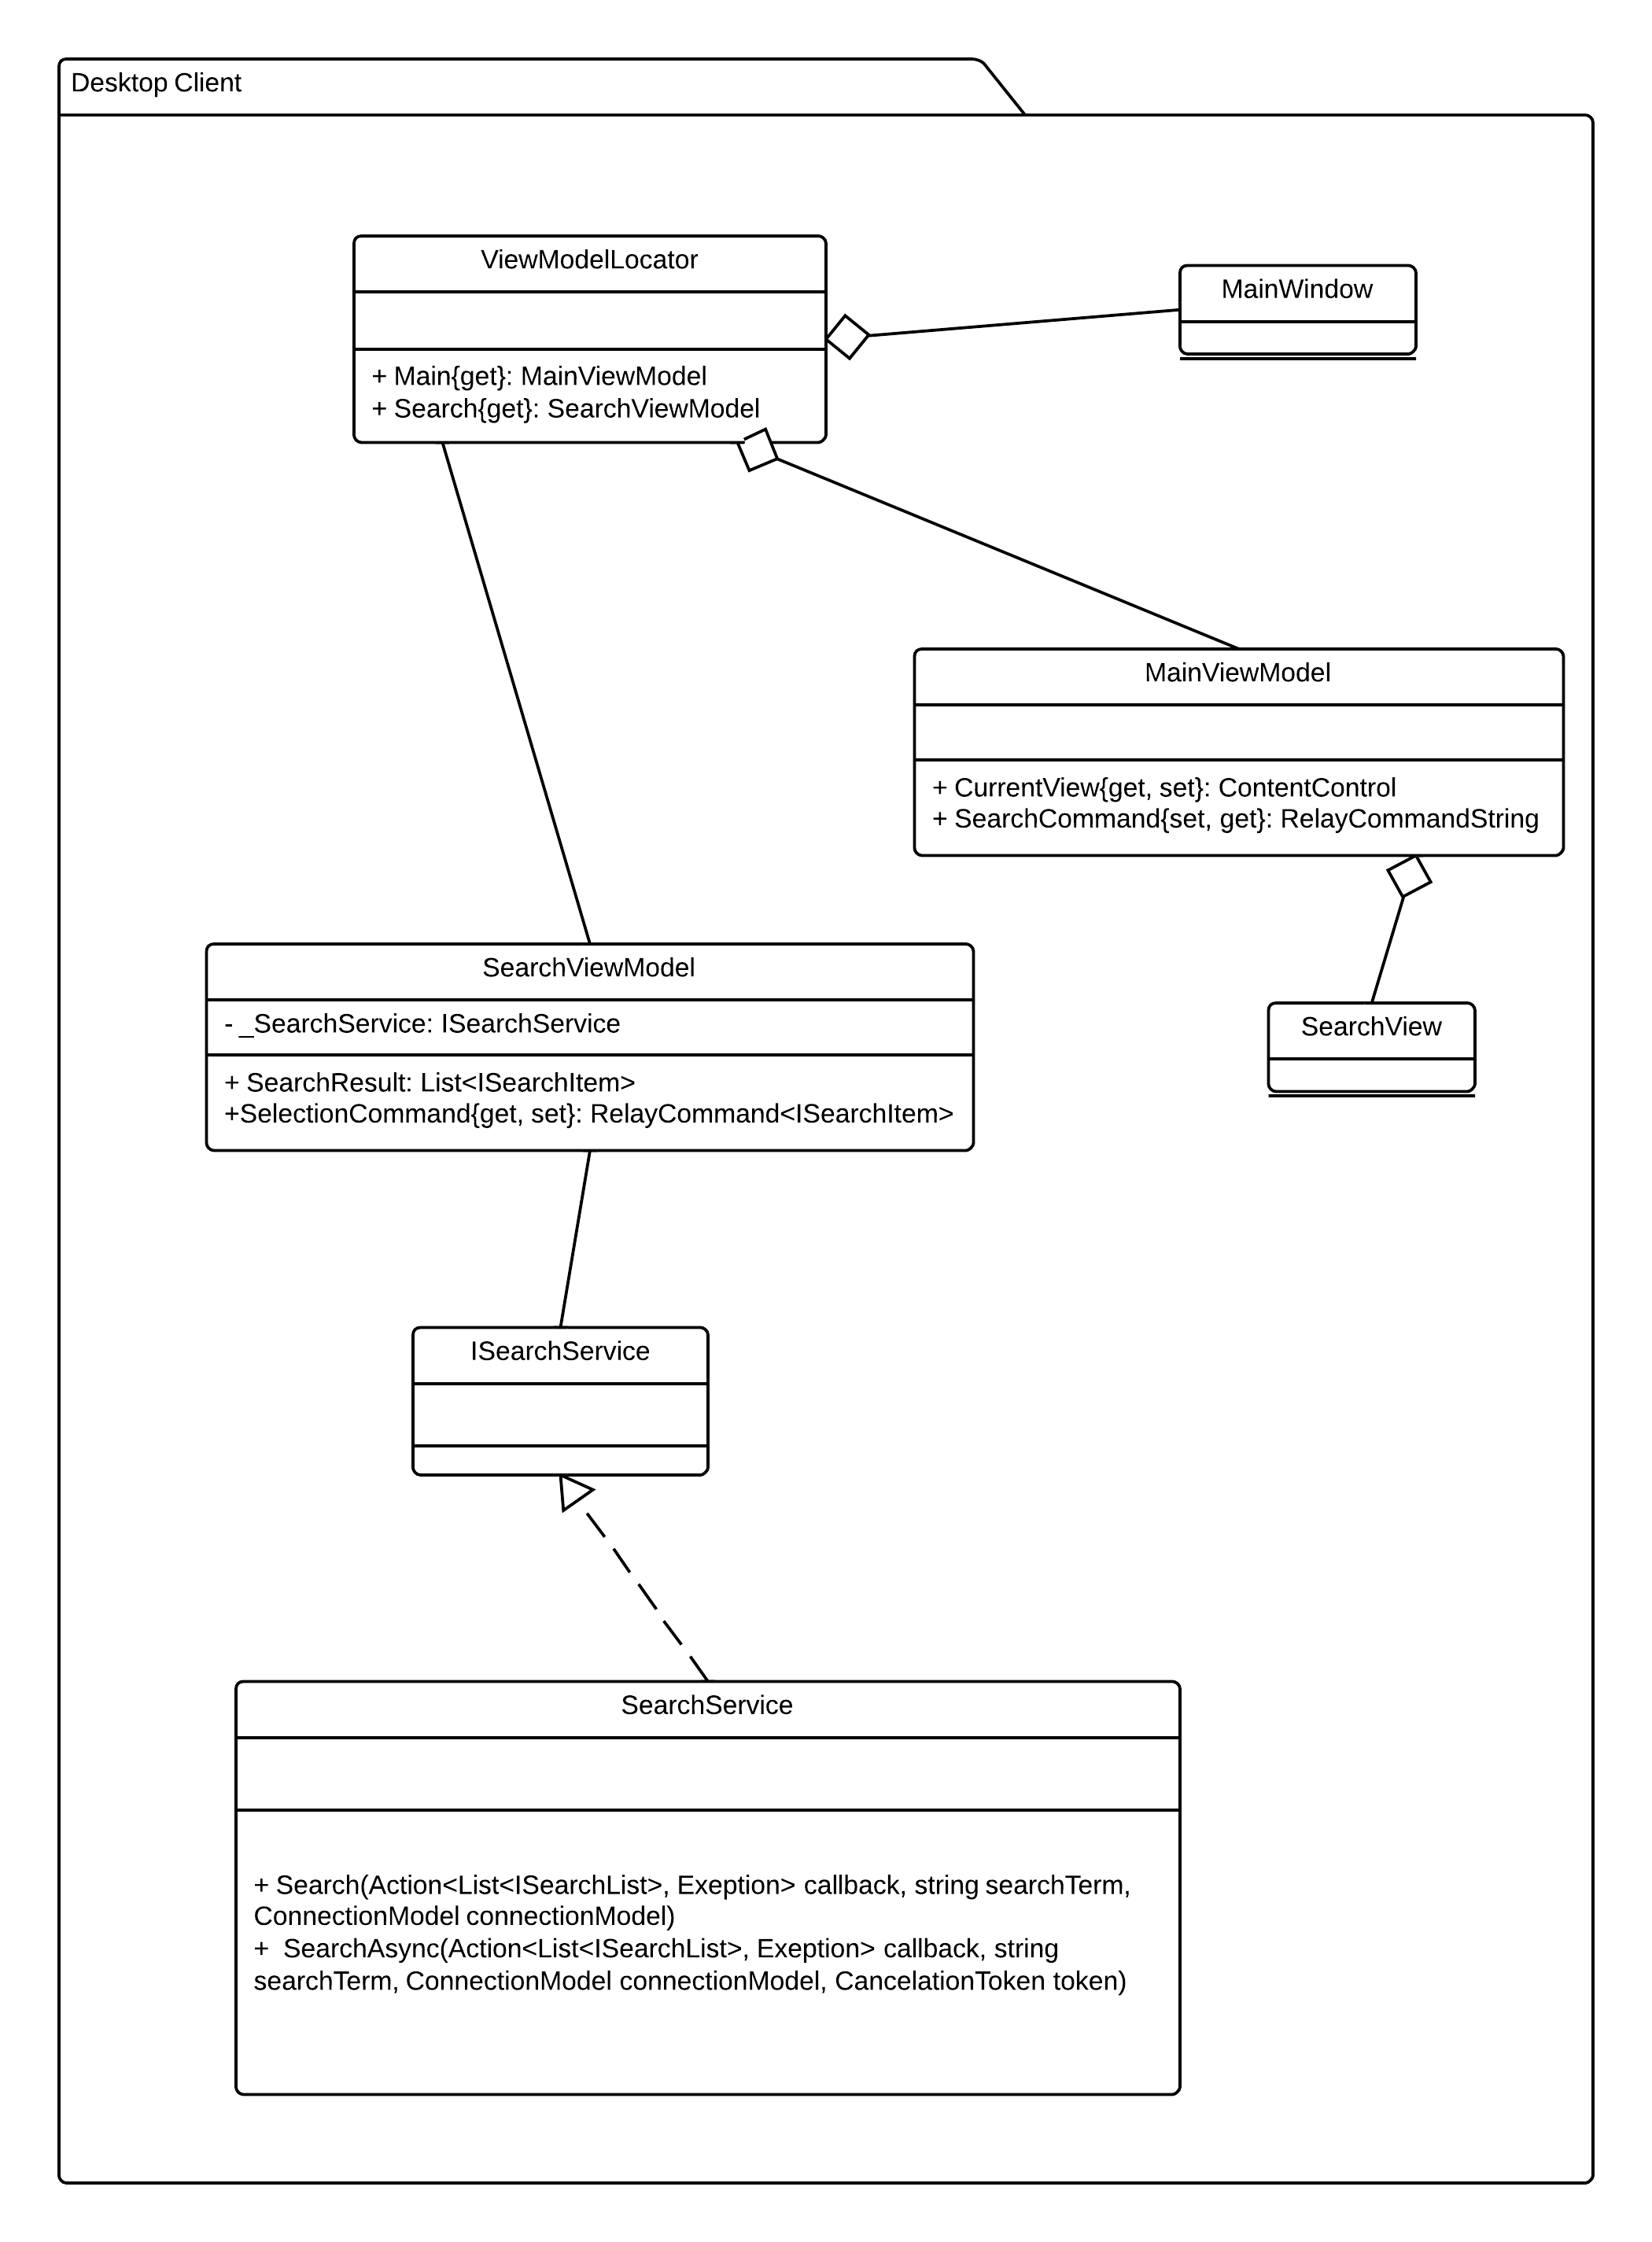
\includegraphics[width=\linewidth]{img/SDD/DesktopClientSubsystem.png}
\caption{DesktopClient subsystem}
\label{fig:DesktopClientSubsystem}
\end{figure}

The desktop client uses the MVVM Light framework to obtain a decoupled MVVM architecture. Views bind to ViewModels through the ViewModelLocator, and ViewModels hold models and other properties to be binded to. Services are injectet into the ViewModels and uses through Messeging and Commands.


\begin{figure}[H]
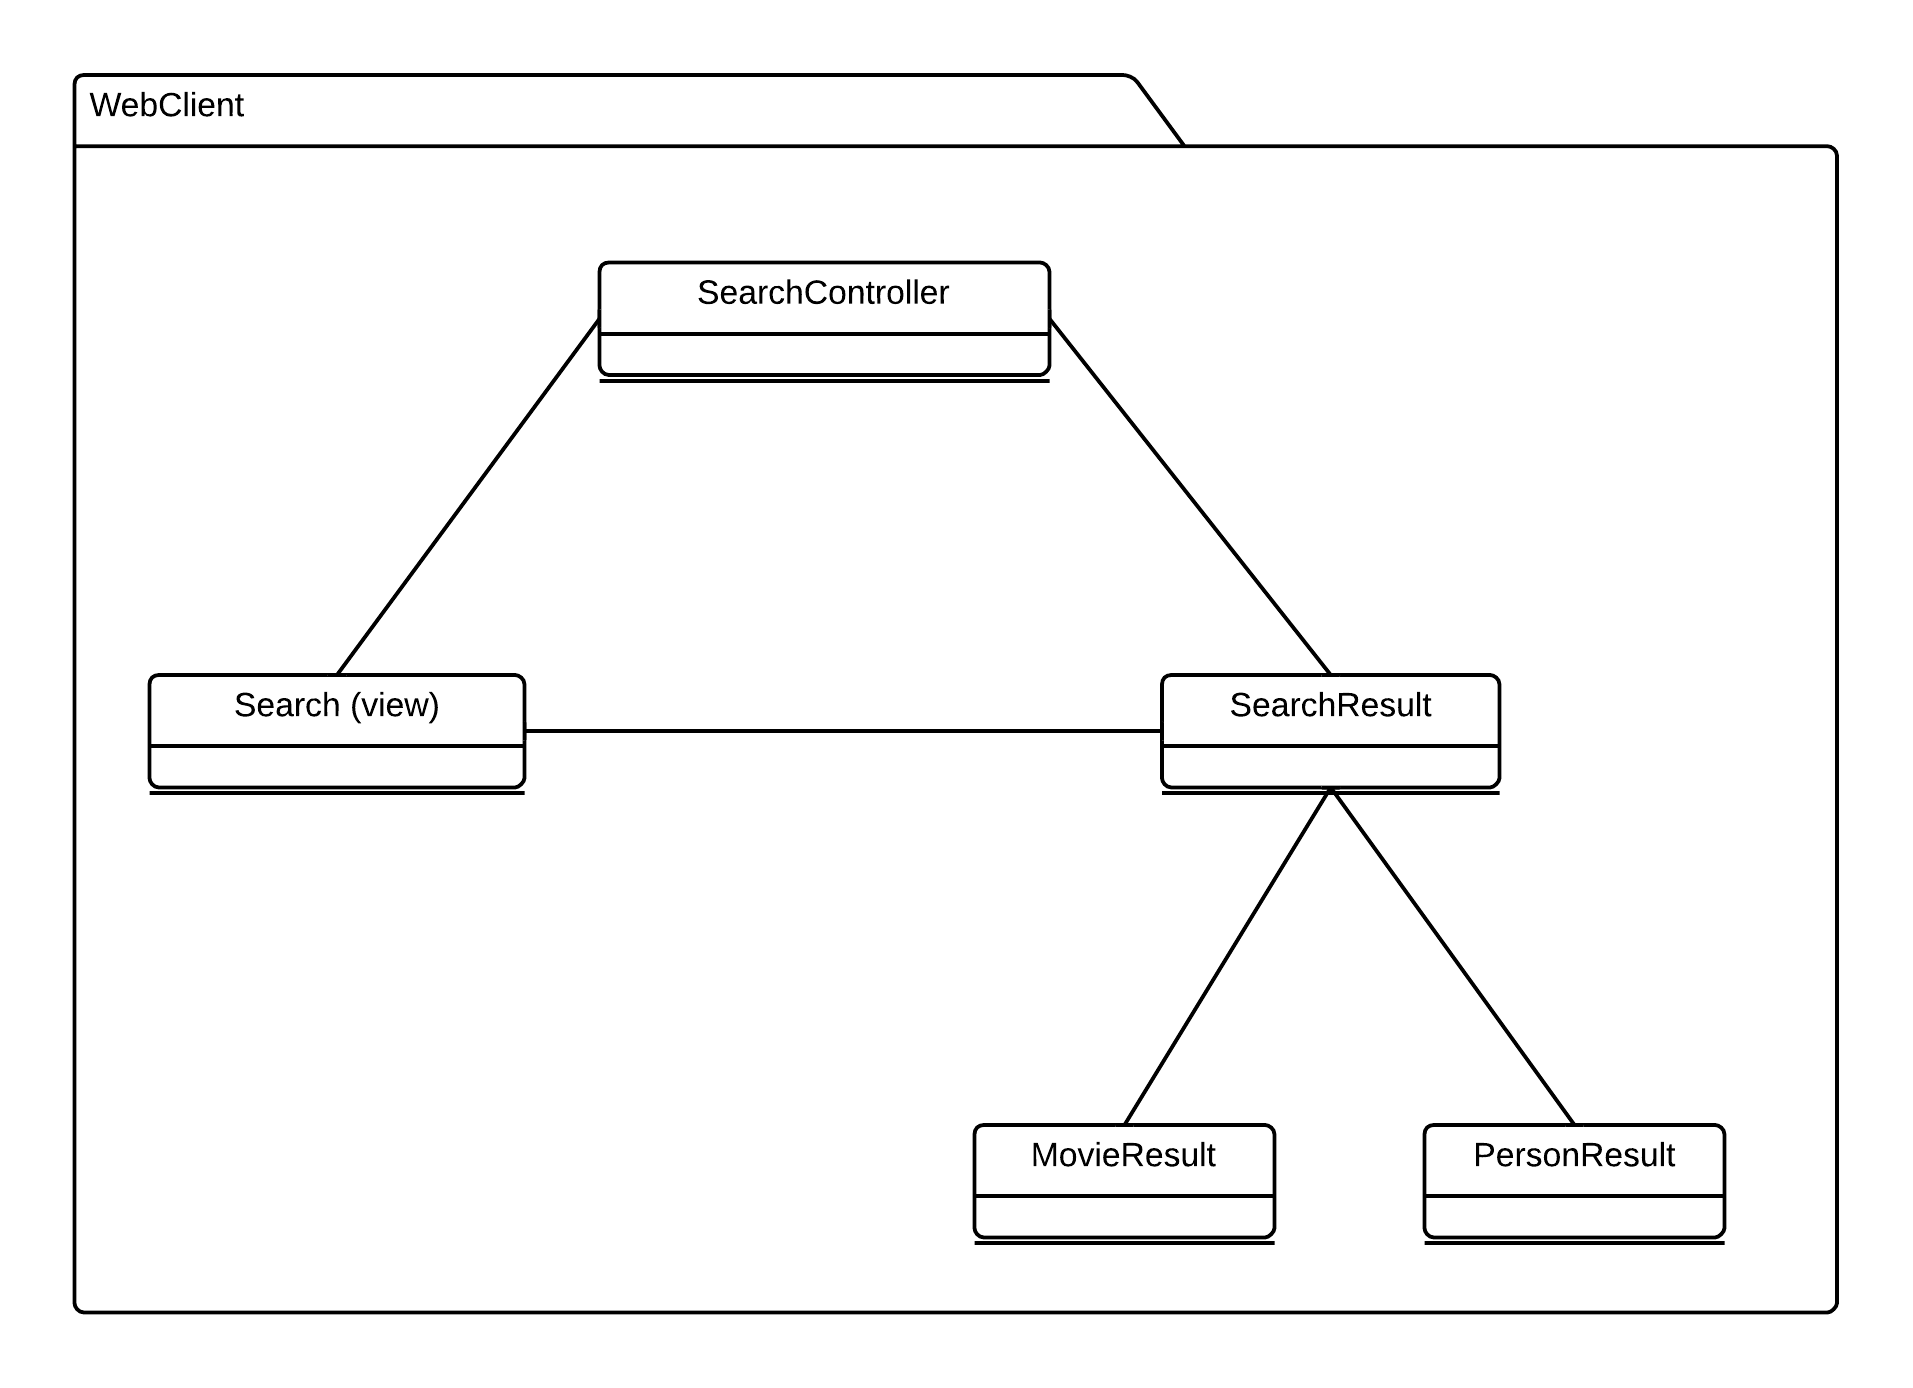
\includegraphics[width=\linewidth]{img/SDD/WebClientSubsystem.png}
\caption{A snippet of the Web Client}
\label{fig:WebClientSubsystem}
\end{figure}

The Web Client utilizes the ASP.Net framework which contains a lot of classes which are redundant to visualize through a common static class diagram. Instead only the classes used when searching is shown. The SearchController uses the SearchResult to get a movieresult or personresult to show in the Search(view)\\

\begin{figure}[H]
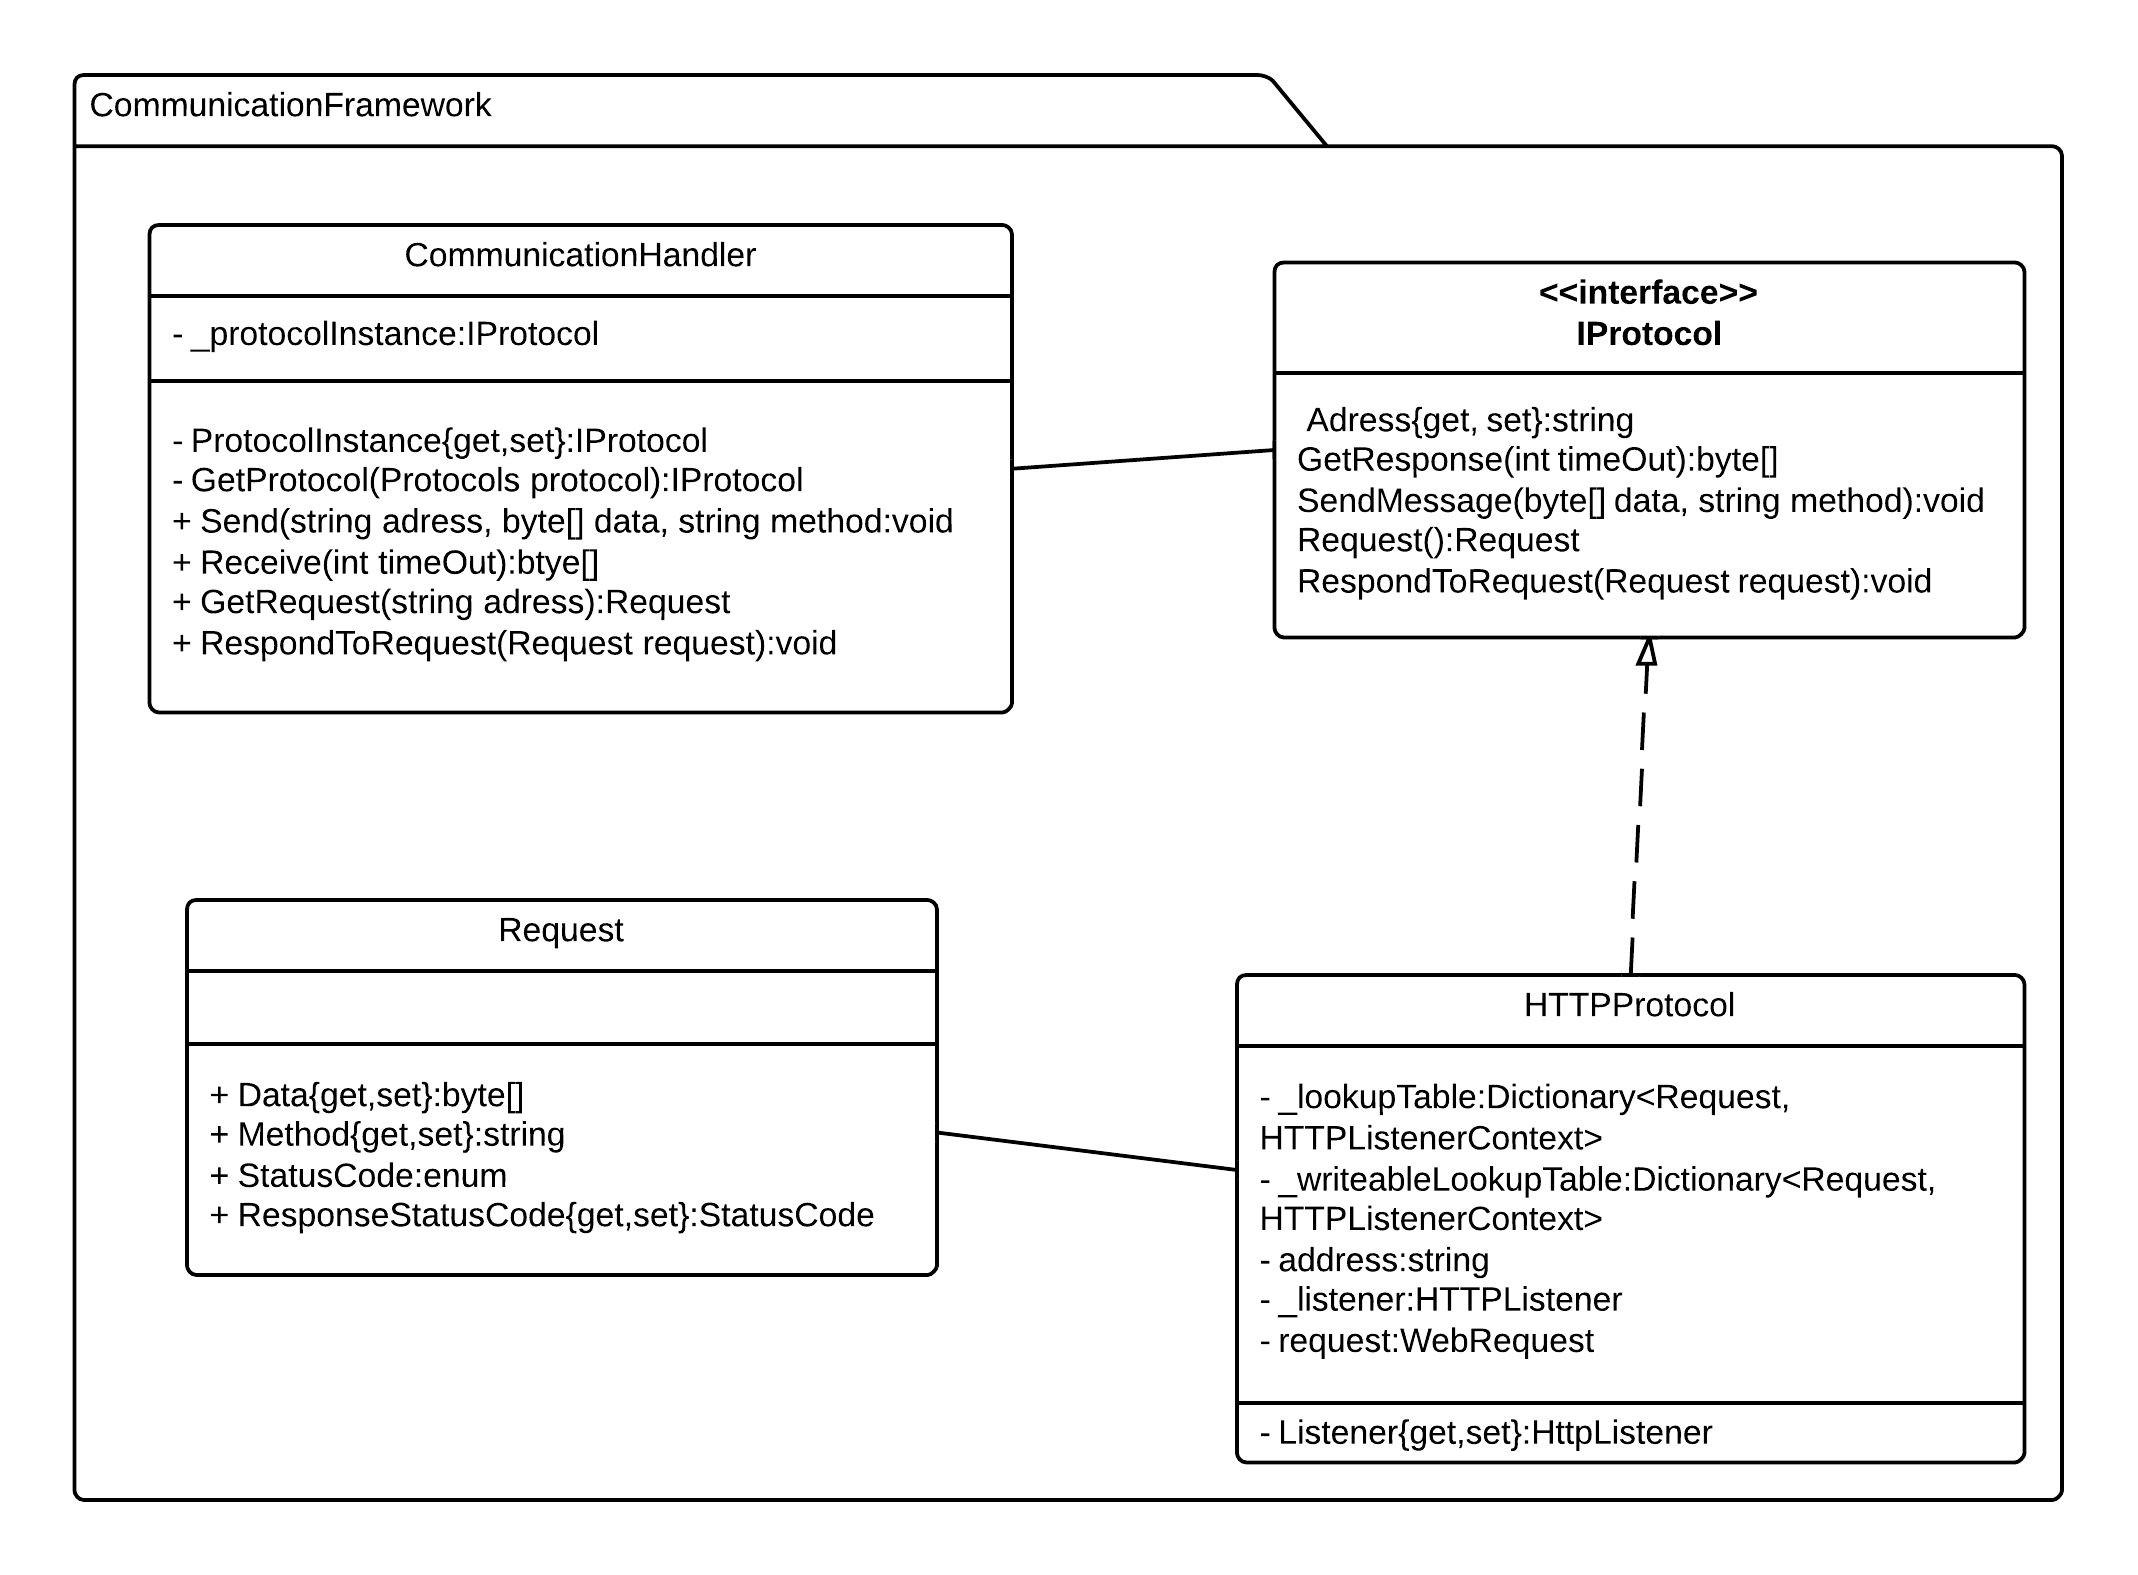
\includegraphics[width=\linewidth]{img/SDD/CommunicationFrameWork.png}
\caption{Communication Framework Subsystem}
\label{fig:CommunicationFramework}
\end{figure}
The communication framework subsystem is used when sending and receiving requests. The framework is used by both the WebServer and each of the clients for communication purposes. The subsystem allows for easy extensibility of more protocol types, though the software at hand only utilizes the Http protocol.

\begin{figure}[H]
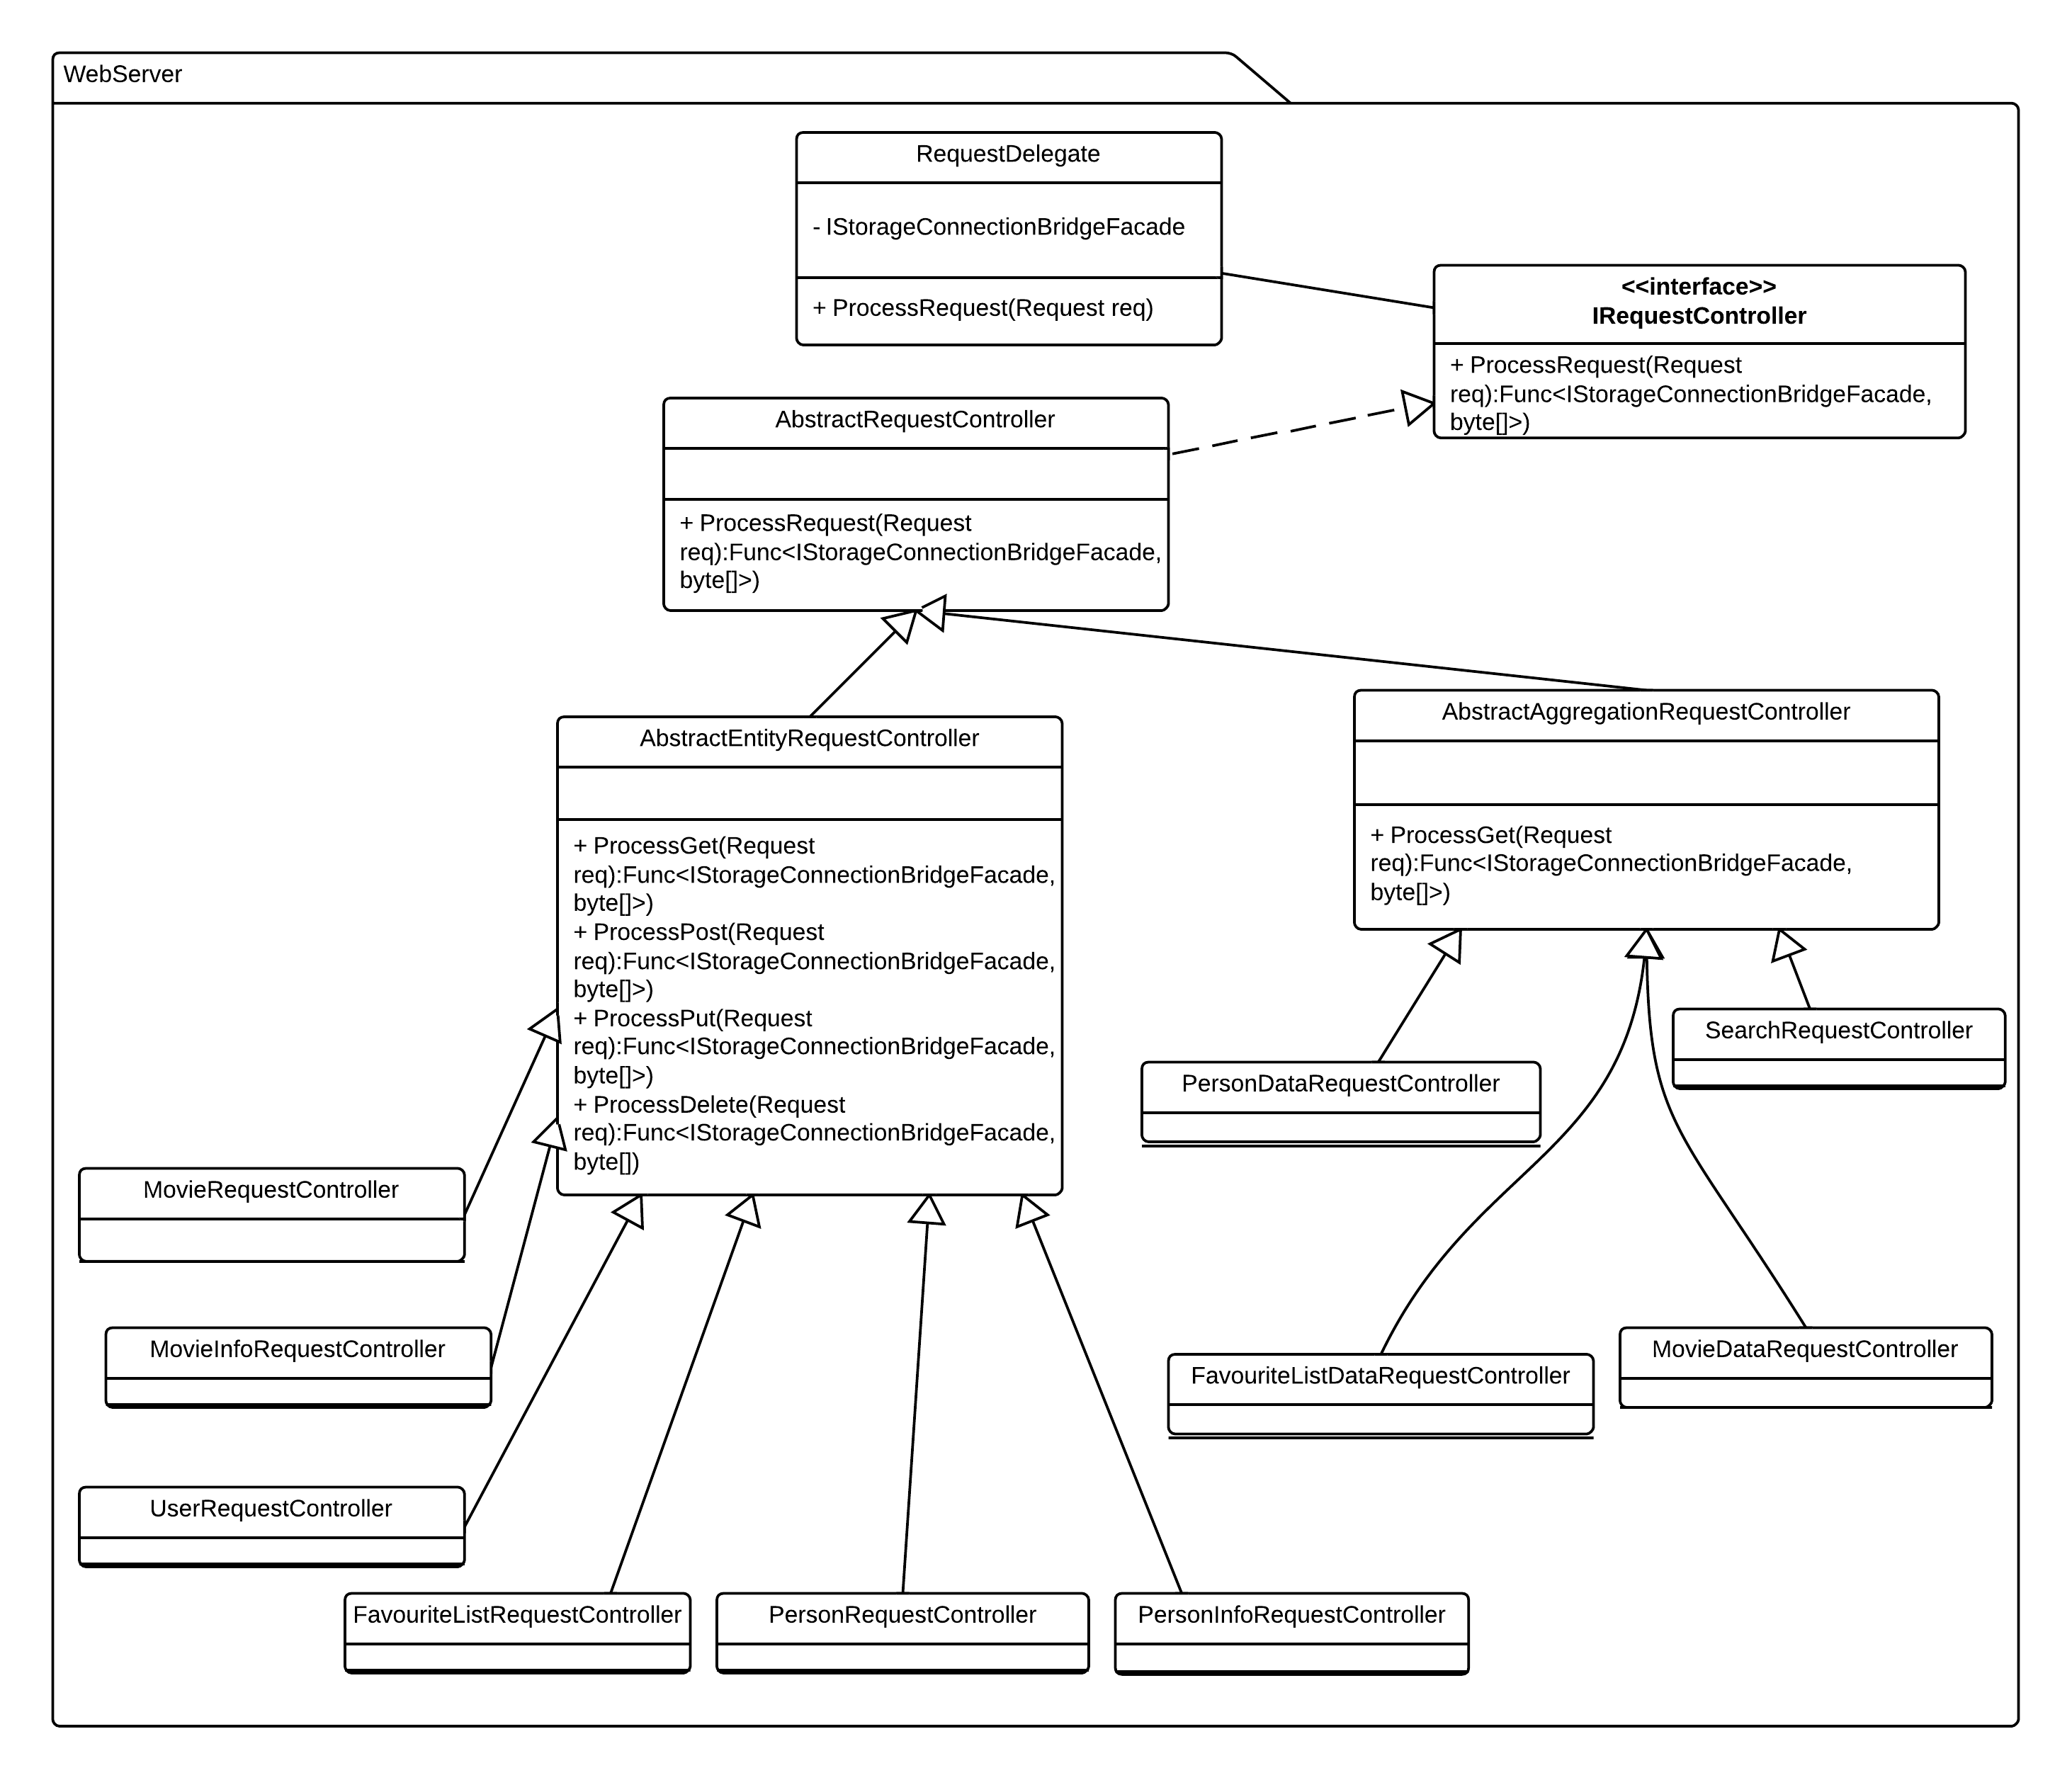
\includegraphics[width=\linewidth]{img/SDD/WebserverSubsystem.png}
\caption{Web Server Subsystem}
\label{fig:WebServer}
\end{figure}
The WebServer is used to interpret incoming requests, received through the communication framework. The requests will be handled by the designated controller (if any exists), or discarded with an error code, since the server is not able to process it any further.
The RequestDelegator facade will use a delegate given by the specified controller to access the database and retrieve or modify the relevant data. When the request has been handled, the WebServer responds to the request using the communication framework.

\begin{figure}[H]
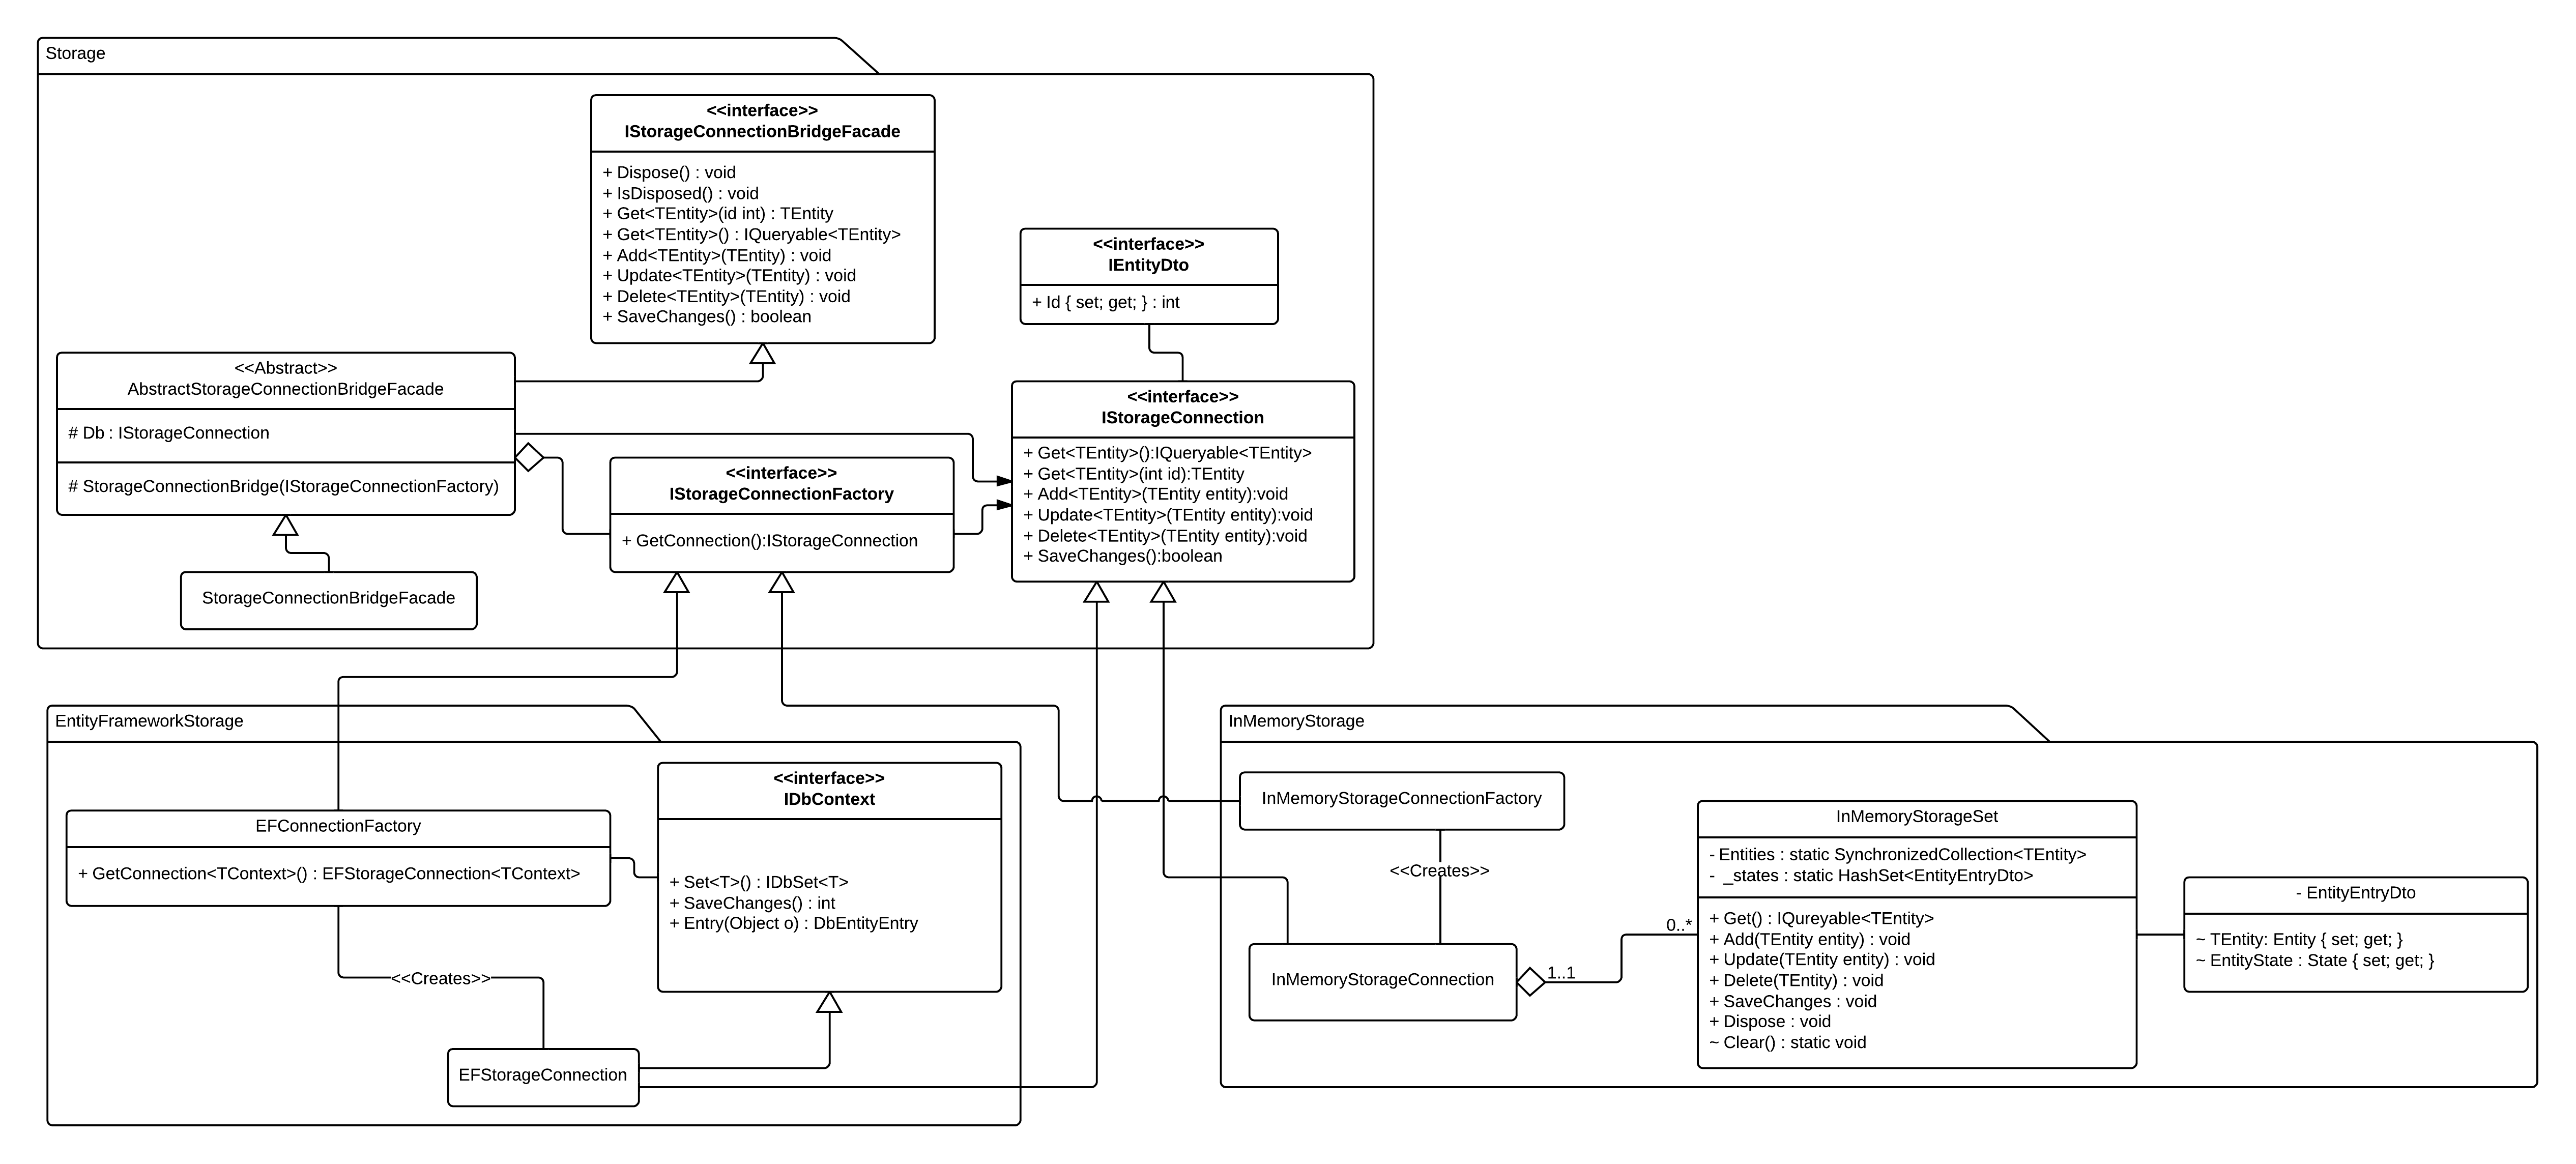
\includegraphics[width=\linewidth]{img/SDD/StoragePackage.png}
\caption{Storage Subsystem}
\label{fig:StorageSubsystem}
\end{figure}

The storage subsystem exposes a bridge facade that allows easy access to the database. The context and the database type (either entity framework or in-memory) is injected through the facade, allowing a generic mapper pattern that doesn't have to know anything about the model being used.

An Abstract factory have been implemented to allow new storage methods to be easily integrated with the existing storage module as it can just be injected into the solution.

\subsection{Hardware/software mapping}
\label{sec:Hardware/software mapping}
Below are the generalized components mapped to hardware or software
\begin{figure}[H]
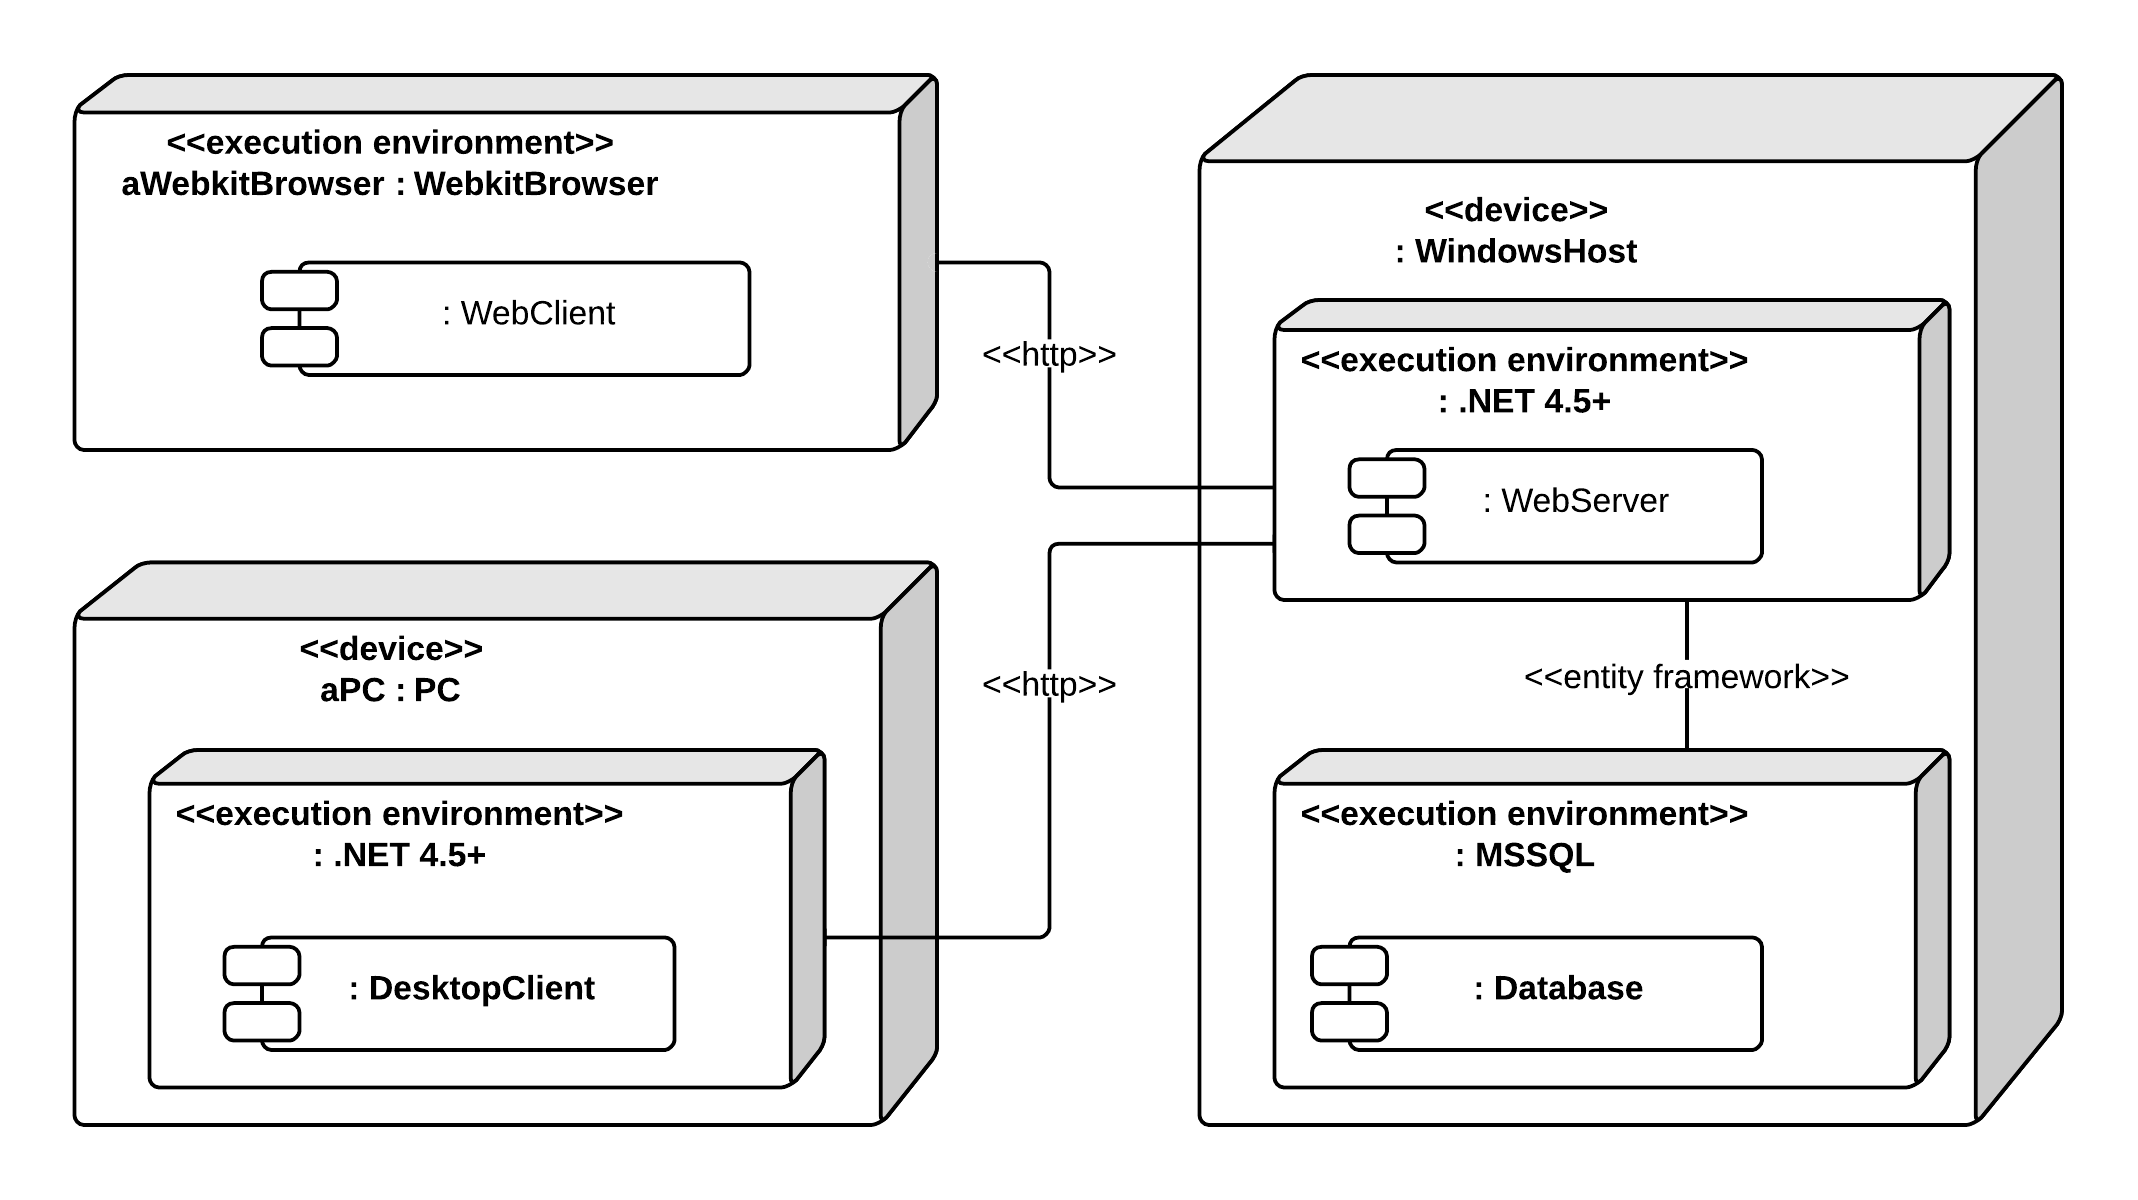
\includegraphics[scale=0.2]{img/SDD/SoftwareHardwareMapping.png}
\caption{Software/Hardware Mapping}
\label{fig:SoftwareHardwareMapping}
\end{figure}

\begin{itemize}
\item \textbf{aPC} is the hardware node for our DesktopClient component. The requirement is that it must run on a PC with Windows 7 or 8, utilizing .NET 4.5 or greater
\item \textbf{aWebkitBrowser} is a software environment implementing WebKit 2 or greater, able to execute our WebClient component. There are no requirements to the hardware platform. This could be any device with a browser powered by WebKit.
\item \textbf{WindowsHost} is the server hardware node. On it are two execution environments: .NET 4.5 or greater and MSSQL, required for our WebServer and Database components respectively. The components communicate by entity framework which allows for moving an environment and component to another WindowsHost hardware node.
\end{itemize}

\subsection{Persistent data management}
\subsubsection{Identifying persistent objects}
The persistent objects for the system is already given and implemented in an MSSQL MDF file. Therefore the system has to adapt the already functional relational database. Some entities have been added to fulfil the use cases of the system, plus to make it easily extendible. See figure \ref{fig:ER Diagram}.

\begin{figure}[H]
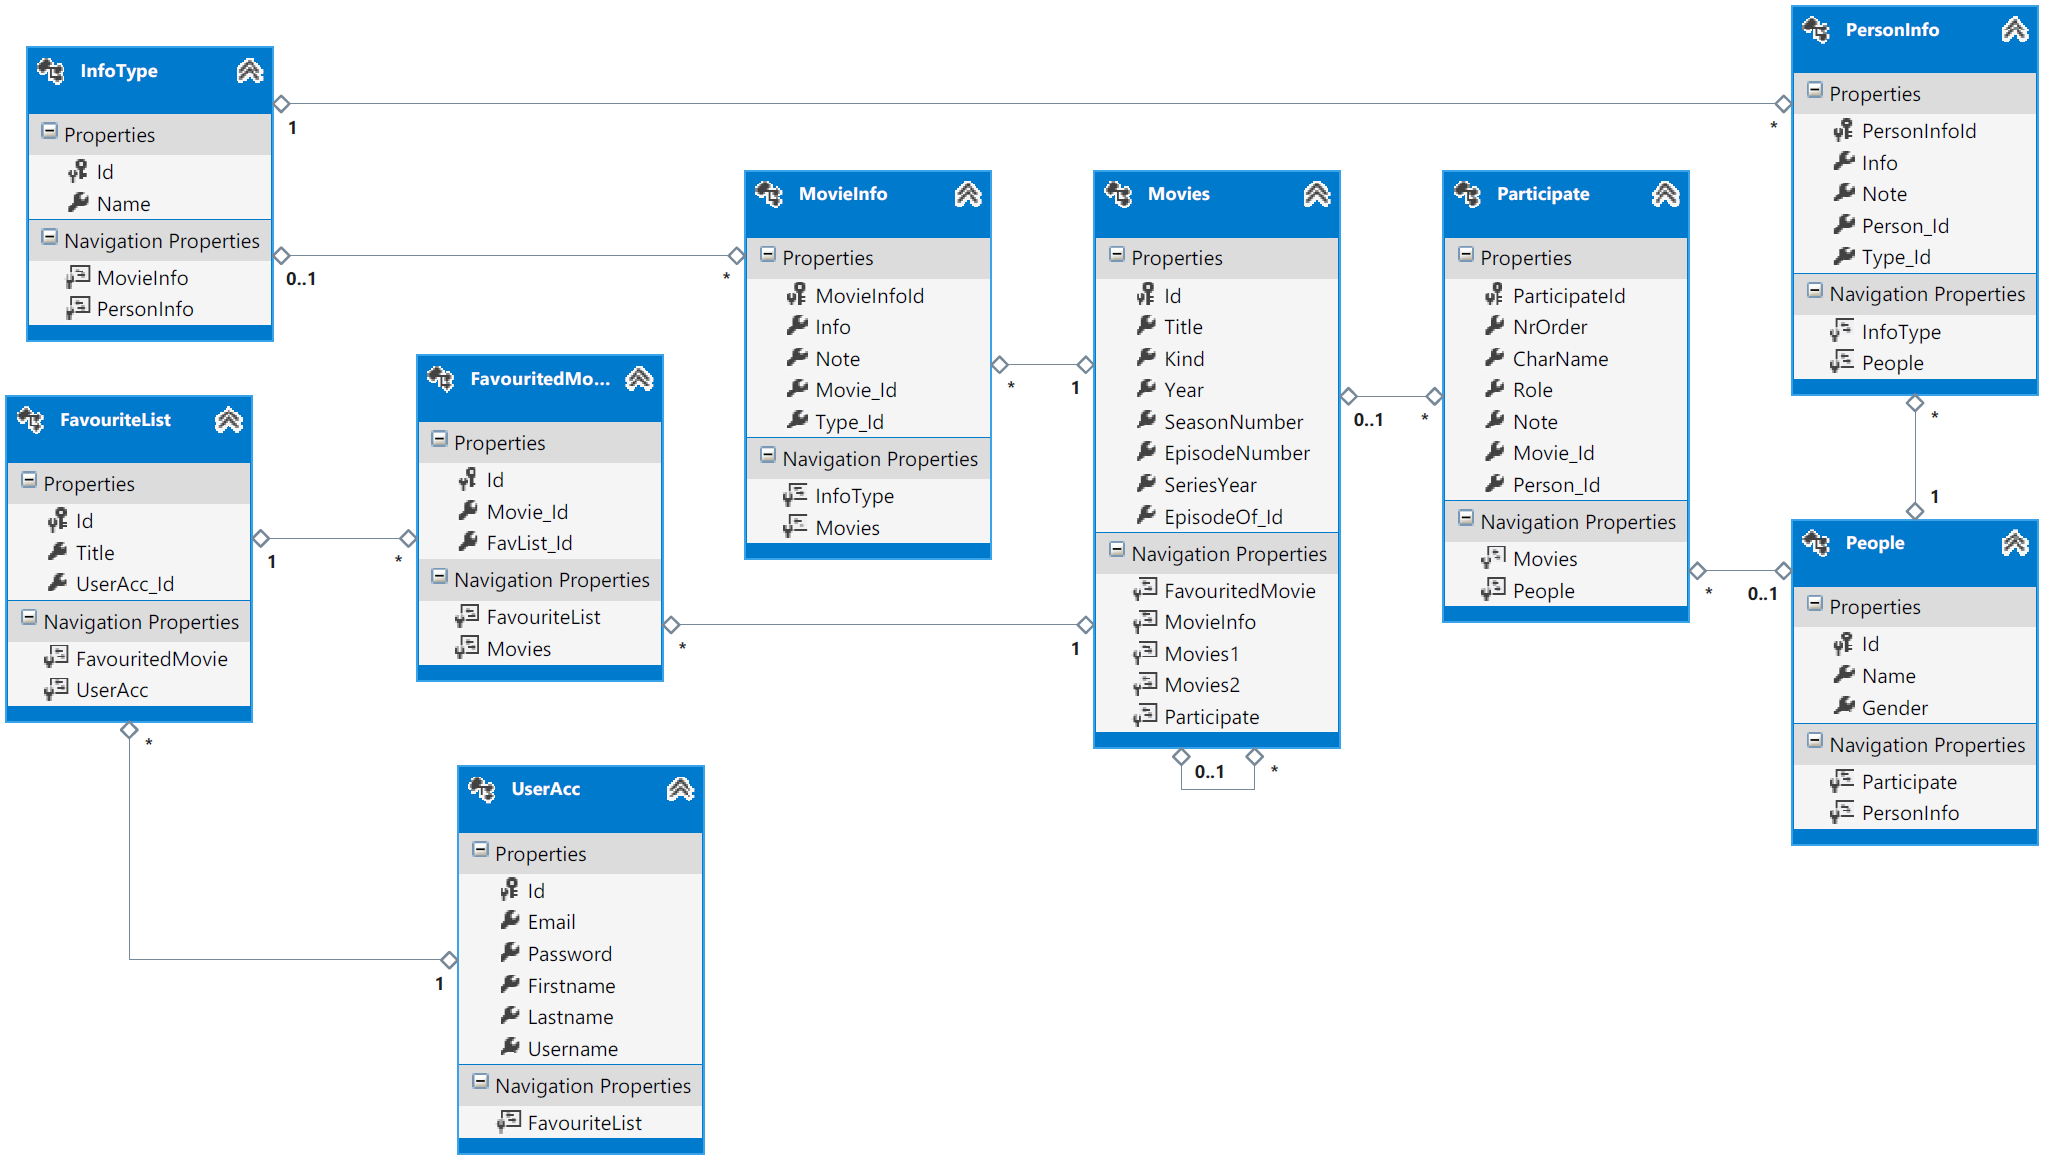
\includegraphics[width=\linewidth]{img/SDD/ER.png}
\caption{Entity relation diagram (ERD)}
\label{fig:ER Diagram}
\end{figure}

\subsubsection{Storage management strategy}
The web server is designed as an layered architecture. On top there's the REST communication, then a logic layer, then a storage layer and on the bottom concrete persistent modules (eg. A database).\\\\
The storage layer is implemented with different design patterns (see figure \ref{fig:StorageSubsystem}), but the overall architecture is built around the object-mapper pattern. This means that the storage layer doesn't know anything about the object model. This is done so that if a new entity were to be added, only the object model has to been updated in order to implement the change. 

The system implements two storage strategies. A relational database management system implemented using Entity Framework, and a proof of concept In-Memory storage solution that could later be used to implement caching. 

Both concrete solutions are using the transaction state pattern to ensure that the database is consistent. The state pattern keeps track of the entities states (see figure ~\ref{fig:Entity State Machine Diagram}), and only when Save Changes is invoked, the data is actually saved to the persistent module. This ensures that if the program were to crash while working on ongoing transactions, the persistent data integrity would not be violated.  

\subsubsection{Relational database}
To improve performance and repose time, we have altered the database to use clustered indexing on key values and non-clustered indexes on often used attributes. Besides that, the database uses foreign keys which the entity framework uses for making property references for easy mapping between objects. 


\subsection{Access control and security}
\begin{itemize}
\item Access Control: The idea with the system is to make a version of IMDb where the users are in control of the content on the site. The system doesn't operate with different levels of access control, since only one type of users exist where everyone is anonymous. All users are able to get, post and edit -information, which means everyone has unlimited access to all data in the system.\\
\item Security: There is no security in the system in the sense of encryption of the messages that are sent back and forth, nor any user control. A user does not log into the system as there is no functionality for accounts in place currently, however the server implementation already has the features necessary to support this feature in a future release.
\end{itemize}

\subsection{Global software control}
The global control flow in our system is primarily designed as an event driven control flow. Whenever the client performs an action, the event is passed on to the WebServer through the Communication Framework. Once the WebServer receives this request, a new thread is started for this particular request and a RequestDelegator is created that will handle the request. The Storage is then invoked by the RequestController that the RequestDelegator has delegated the request to. This allows parellel handling of the requests and is a very responsive system making it possible to respond to other requests while several are being processed at the same time and the only limit to the amount of concurrenct users is the amount of processing power that is available. Once a request has been handled by the WebServer and the response is ready, it's sent back through the Communication Framework to the client, waiting for the response. 

\subsection{Identifying services}
We have identified subsystem services for our program. They are shown in the figure below, and more detailed explanations for the services can be found beneath the diagram.

\begin{figure}[H]
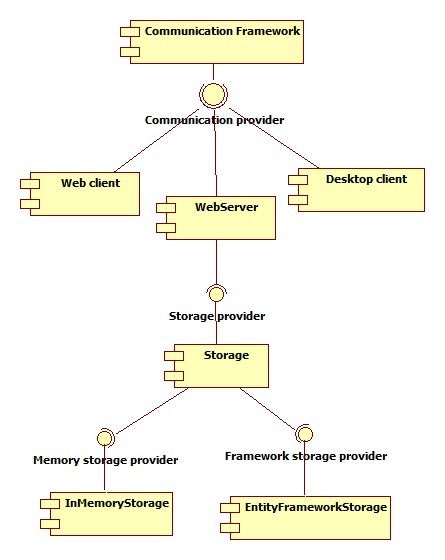
\includegraphics[scale=0.8]{img/SDD/SubsystemServices.jpg}
\caption{Subsystem Services}
\label{fig:Subsystem Services}
\end{figure}


\begin{itemize}
	\item Communication provider, which provides the clients and webserver with access to the communication framework, allowing them to send messages to each other.
	\item Storage provider, which provides the webserver with the methods required to get information / post information to the database.
	\item Framework storage provider, which provides the storage subsystem with the methods needed to store entities in-memory.
	\item Memory storage provider, which provides the storage subsystem with the methods required for storing entities via the entity framework.
\end{itemize}

\subsection{Boundary conditions}

We have identified the following boundary conditions and added them to the list of use cases in the RAD:

\begin{itemize}
	\item Start up and shutdown boundary use cases:
	\begin{itemize}
			\item StartWebServer
			\item ShutdownWebServer
	\end{itemize}
	\item Exception use cases:
	\begin{itemize}
			\item ServerCrashException
			\item ConnectionLostException
	\end{itemize}
\end{itemize}

\subsection{Identifying optimization possibilities}

The software under development has a high degree of finality though there are always ways of optimizing the end product.
When considering optimizations there are two fields of extensibility at hand.

\subsubsection{Features}

The end product contains many features, yet some improvements could have been made.
The features being mentioned are the ones slightly beyond scope, yet within reach of another week of development.

- Additional features exposed through clients
The backend of the program exposes services to manage the entire database in an easy fashion. These services are however not fully utilized in the clients, due to the complications of developing a rich user interface that exposes each of the services in a decent way.

- Improved Caching
Even though the entity framework supports minor caching, the respond times of the web server could greatly be improved by caching various resources.
The main methods of caching, currently under discussion, is entity caching in which the server would cache any resources being exposed through a request for later use, or query caching, in which a query's result would be stored locally.

\subsubsection{Optimization}

The software being developed, even though it already has a high amount of quality checks and revisions, can always be improved.
The optimization options being mentioned are those of code optimization, speed optimization or structure optimization in general.

- Json messaging
The software communicates through the use of json. The json is stored as a single json object with various attribute names and attribute values.
The communication could be improved to use actual json objects, while using anonymous and dynamic objects for serializing and deserializing, to prevent a static structure, in which no server and client version can be out of sync.

- Communication Framework
The communication framework was specifically designed to be easily expandable with additional protocol types. The internal structure of the subsystem has a lot of logic that could be shared between protocols, being defined in the http protocol class structure. This logic should be moved to a higher level, for easier sharing between polymorphic members.

- Higher quality of testing
In general the amount of tests being conducted on each individual subsystem was too insignificant. More thorough testing should be conducted to better validate the correctedness of the software.


\chapter{Discussion}

\chapter{SCRUM}
For the main part of this project, we have worked as a SCRUM unit. It has helped us work more effectively as a unit but with certain challenges.

\begin{itemize}
\item In our experience, not having a central base, is a big hit on SCRUM. It means that we weren't able to have a physical SCRUM board, and were forced to use a mobile tool. We chose to use Trello, where each of us could log in, check up on and move tasks. The idea is fine, but easily forgotten. Today is our last scheduled work day, and we have transformed the tasks on post-its(see \ref{fig:Scrum Board1} page \pageref{fig:Scrum Board1}). To sum up, a physical board achieved being the status of progress, while Trello was more of another task to keep updated.
\end{itemize}

\section{Extreme programming}


\section{Coding priorities}
Our goal form the start was quality over quantity. We realize now that we could have displayed that nicely in the RAD and SDD, and since we haven't, it might seem like many usecases wasn't achieved. Instead we could have focused more on a requirement to supportability and extensibility, which we have achieved.
We have focused on the architecture on all fronts. We began with the backend, using a wide variety of design patterns and building a framework for communication. The same goes for the clients - however since we were working against a strict deadline, our clients did not get to reflect the full functionality of the backend. Our time was rather spent on the architecture of them. However our backend has controls for RESTful calls on all tables in the database. 
